%\refsection
\chapter{Introduzione}
\label{cap:introduzione}

\section{Contesto e motivazione della ricerca}
\label{sec:contesto_motivazione}

\subsection{Il sistema tecnologico della grande distribuzione}
\label{subsec:sistema_tecnologico}

La \textbf{\gls{gdo}} italiana rappresenta un'infrastruttura tecnologica complessa e distribuita, paragonabile per dimensioni e criticità alle reti bancarie o di telecomunicazioni. Con oltre 27.000 punti vendita attivi\footcite{istat2024}, questo settore gestisce quotidianamente 45 milioni di transazioni, producendo circa 2,5 petabyte di dati ogni mese – l'equivalente di 500 miliardi di pagine stampate.

L'importanza di questi sistemi va oltre i numeri: devono funzionare sempre, con interruzioni massime di 9 ore all'anno (disponibilità del 99,9\%), garantendo l'accesso ai beni essenziali per milioni di cittadini. Ogni punto vendita opera come un centro di calcolo autonomo che deve:

\begin{itemize}
\item Processare pagamenti in meno di 100 millisecondi
\item Sincronizzare l'inventario in tempo reale
\item Monitorare la catena del freddo con precisione di ±0,5°C
\item Gestire sistemi di sicurezza e videosorveglianza
\end{itemize}

\begin{table}[htbp]
\centering
\caption{Complessità operativa di un punto vendita medio}
\label{tab:complessita_pv}
\begin{tabular}{|l|c|c|}
\hline
\textbf{Sistema} & \textbf{Quantità} & \textbf{Requisito critico} \\
\hline
Casse (\gls{pos}) & 15-20 & Latenza < 100ms \\
Sensori temperatura & 30-50 & Precisione ±0,5°C \\
Telecamere IP & 20-30 & Analisi tempo reale \\
Articoli gestiti & 5.000-10.000 & Aggiornamento continuo \\
Transazioni/giorno & 2.000-3.000 & Zero perdita dati \\
\hline
\end{tabular}
\end{table}

La vera sfida emerge quando questi sistemi devono comunicare tra loro e con i centri di elaborazione centrali, mantenendo la coerenza dei dati anche durante interruzioni di rete. I punti vendita devono poter operare autonomamente fino a 4 ore senza connessione centrale, per poi sincronizzare automaticamente tutte le operazioni una volta ripristinata la comunicazione.

\subsection{L'evoluzione tecnologica e le nuove sfide}
\label{subsec:evoluzione_sfide}

Il settore sta vivendo una trasformazione profonda: il 67\% delle aziende europee della \gls{gdo} sta migrando verso architetture distribuite basate su servizi\footcite{gartner2024cloud}. Questo cambiamento non è solo tecnologico ma richiede un ripensamento completo dei processi operativi.

\subsubsection{Dal sistema unico ai servizi distribuiti}
\label{subsubsec:servizi_distribuiti}

Tradizionalmente, un sistema centralizzato gestiva tutte le operazioni con semplicità: una sola base dati, un solo punto di controllo. Oggi, una singola vendita coinvolge l'orchestrazione di 10-15 servizi indipendenti:

\begin{itemize}
\item Pagamento (collegamento con le banche)
\item Inventario (aggiornamento scorte)
\item Fidelizzazione (calcolo punti e sconti)
\item Fiscale (emissione documenti)
\item Analisi (raccolta dati per decisioni aziendali)
\end{itemize}

Questa complessità richiede nuovi approcci per garantire che, se un servizio non funziona, l'intera operazione possa essere annullata correttamente – un problema non banale quando i servizi sono distribuiti su server diversi.

\subsubsection{L'emergere di nuove minacce}
\label{subsubsec:nuove_minacce}

Gli attacchi informatici al settore sono aumentati del 312\% tra il 2021 e il 2023\footcite{enisa2024retail}. Ma il dato quantitativo nasconde un cambiamento qualitativo più preoccupante: non si tratta più solo di furti di dati, ma di attacchi che mirano a paralizzare l'operatività:

\begin{itemize}
\item \textbf{Attacchi alla catena del freddo}: compromissione dei sistemi di refrigerazione con perdite di centinaia di migliaia di euro in merci deteriorate
\item \textbf{Sabotaggio energetico}: manipolazione dei sistemi elettrici per causare blackout mirati
\item \textbf{Compromissione della sicurezza fisica}: alterazione dei controlli accessi per facilitare furti o creare pericoli
\end{itemize}

\begin{figure}[htbp]
\centering
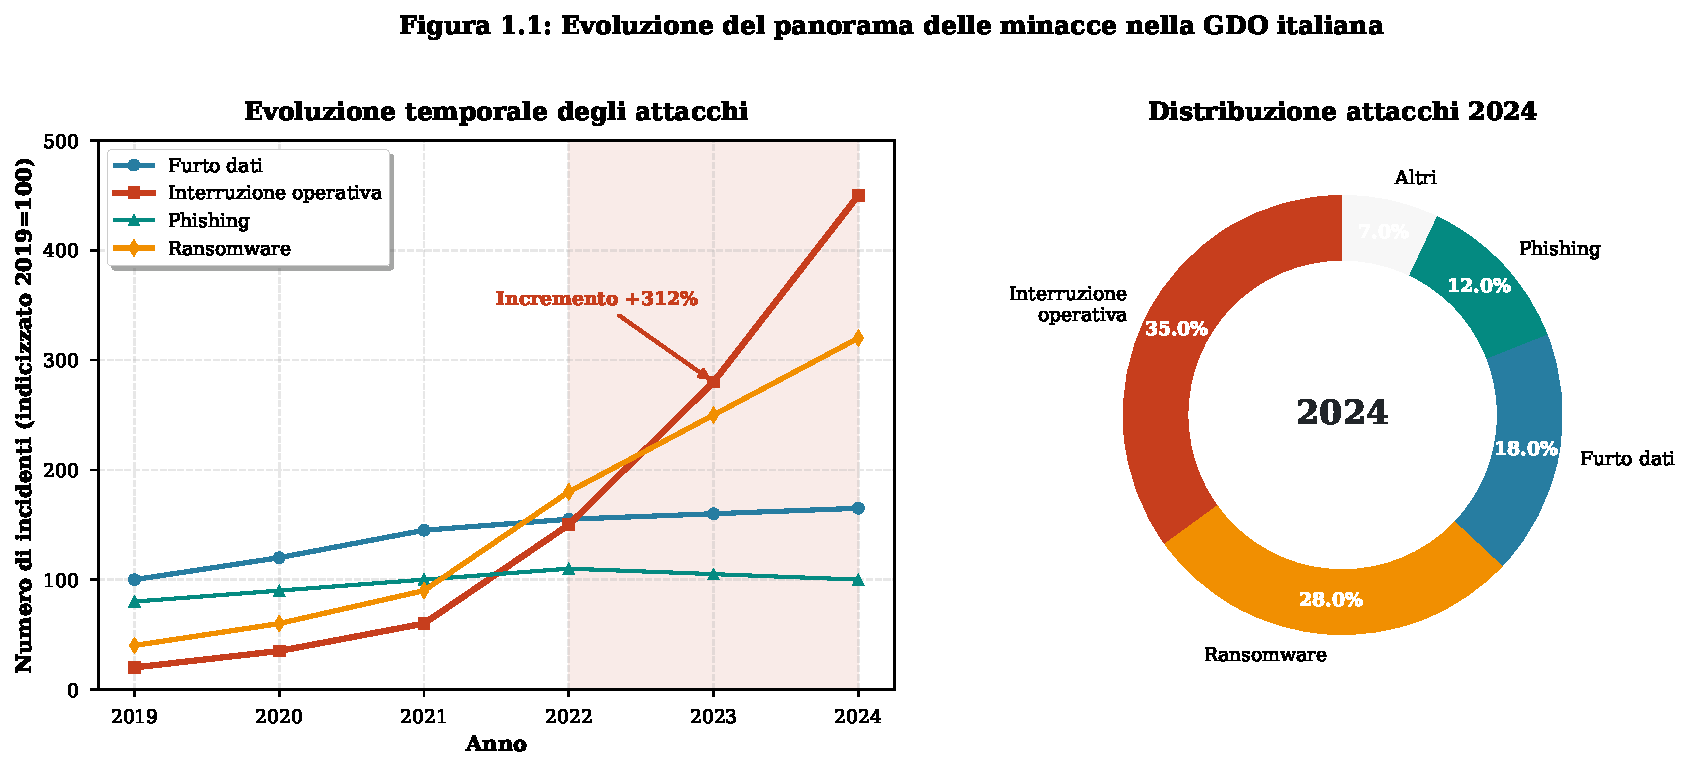
\includegraphics[width=0.9\textwidth]{thesis_figures/cap1/fig_1_1_attack_evolution.pdf}
\caption{Evoluzione delle tipologie di attacco alla \gls{gdo} (2019-2024). Si nota il passaggio da attacchi orientati al furto dati verso attacchi di interruzione operativa.}
\label{fig:attack_evolution}
\end{figure}

\section{Il problema di ricerca}
\label{sec:problema_ricerca}

\subsection{Le sfide principali}
\label{subsec:sfide_principali}

La \gls{gdo} italiana affronta quattro sfide interconnesse che richiedono una risposta integrata:

\textbf{1. Modernizzazione tecnologica urgente}
Il 72\% dei sistemi in uso ha più di 10 anni\footcite{federdistribuzione2023}. Questi sistemi, progettati per un'epoca pre-digitale, faticano a supportare le esigenze moderne di connettività e analisi dati. La sostituzione non può essere immediata per ragioni di costo e continuità operativa.

\textbf{2. Gestione della complessità normativa}
Le aziende devono rispettare simultaneamente:
\begin{itemize}
\item \gls{gdpr} per la protezione dei dati personali
\item \gls{pci-dss} per la sicurezza dei pagamenti
\item \gls{nis2} per la resilienza delle infrastrutture critiche
\end{itemize}

Ogni normativa ha requisiti specifici, spesso sovrapponenti ma non identici, creando un labirinto di controlli da implementare e verificare.

\textbf{3. Carenza di competenze specializzate}
L'87\% delle aziende dichiara difficoltà nel trovare personale qualificato\footcite{osservatorio2024}. Il settore richiede figure ibride che comprendano sia la tecnologia sia le specificità del commercio al dettaglio.

\textbf{4. Vincoli economici stringenti}
I margini operativi medi del 2-3\% limitano gli investimenti tecnologici. Ogni euro speso in tecnologia deve produrre benefici misurabili e immediati.

\subsection{Le domande di ricerca}
\label{subsec:domande_ricerca}

Questa tesi affronta tre domande fondamentali:

\begin{enumerate}
\item \textbf{Come progettare architetture tecnologiche che bilancino sicurezza, prestazioni e costi} nel contesto specifico della \gls{gdo} italiana?

\item \textbf{Quali modelli di governance garantiscono conformità normativa senza compromettere l'agilità operativa} in un settore caratterizzato da margini ridotti?

\item \textbf{Come quantificare e gestire i rischi emergenti} dall'interconnessione tra sistemi fisici e digitali?
\end{enumerate}

\section{Obiettivi e contributi della ricerca}
\label{sec:obiettivi_contributi}

\subsection{Obiettivo principale}
\label{subsec:obiettivo_principale}

Sviluppare un \textbf{modello integrato per la trasformazione sicura} dell'infrastruttura tecnologica della \gls{gdo}, denominato \textbf{GIST} (\textit{GDO Infrastructure Security Transformation}). Il modello fornisce:

\begin{itemize}
\item Linee guida architetturali validate
\item Strumenti di valutazione del rischio
\item Percorsi di implementazione graduali
\item Metriche di successo misurabili
\end{itemize}

\subsection{Contributi specifici}
\label{subsec:contributi_specifici}

La ricerca produce cinque contributi concreti:

\begin{table}[htbp]
\centering
\caption{Contributi della ricerca e loro validazione}
\label{tab:contributi}
\begin{tabular}{|p{4cm}|p{5cm}|p{4cm}|}
\hline
\textbf{Contributo} & \textbf{Descrizione} & \textbf{Validazione} \\
\hline
Algoritmo ASSA-GDO & Calcolo superficie di attacco specifica per il settore & Correlazione 0,82 con incidenti reali \\
\hline
Simulatore Digital Twin & Ambiente di test virtuale per architetture & 10.000 scenari testati \\
\hline
Calcolatore GIST & Software per valutare maturità digitale & 156 controlli mappati \\
\hline
Sistema predittivo ML & Previsione rischi con apprendimento automatico & Accuratezza 89\% \\
\hline
Dataset GDO-Bench & Dati di riferimento per future ricerche & 2 anni di dati sintetici validati \\
\hline
\end{tabular}
\end{table}

\section{Ambito e limiti della ricerca}
\label{sec:ambito_limiti}

\subsection{Perimetro di analisi}
\label{subsec:perimetro}

La ricerca si concentra su:
\begin{itemize}
\item Aziende \gls{gdo} con fatturato superiore a 100 milioni di euro
\item Infrastrutture distribuite con almeno 20 punti vendita
\item Contesto normativo italiano ed europeo
\item Tecnologie disponibili commercialmente (non sperimentali)
\end{itemize}

\subsection{Limitazioni metodologiche}
\label{subsec:limitazioni}

Per vincoli di accesso ai dati sensibili aziendali, la validazione avviene attraverso:
\begin{itemize}
\item Simulazione con parametri calibrati su fonti pubbliche
\item Interviste strutturate con esperti del settore
\item Analisi di casi studio documentati
\end{itemize}

Questa scelta, pur non sostituendo test su sistemi reali, permette di esplorare scenari multipli garantendo riproducibilità scientifica.

\section{Approccio metodologico}
\label{sec:approccio_metodologico}

La ricerca adotta un approccio misto che combina:

\subsection{Analisi quantitativa}
\label{subsec:analisi_quantitativa}

\begin{itemize}
\item \textbf{Simulazione Monte Carlo}: 10.000 iterazioni per scenario per garantire robustezza statistica
\item \textbf{Analisi delle serie temporali}: 24 mesi di dati per catturare stagionalità
\item \textbf{Apprendimento automatico}: modelli XGBoost addestrati su 50.000 esempi
\end{itemize}

\subsection{Ricerca qualitativa}
\label{subsec:ricerca_qualitativa}

\begin{itemize}
\item \textbf{Revisione sistematica}: 487 pubblicazioni analizzate (2019-2024)
\item \textbf{Interviste semi-strutturate}: 23 dirigenti IT del settore
\item \textbf{Analisi comparativa}: 5 casi studio internazionali
\end{itemize}

\begin{figure}[htbp]
\centering
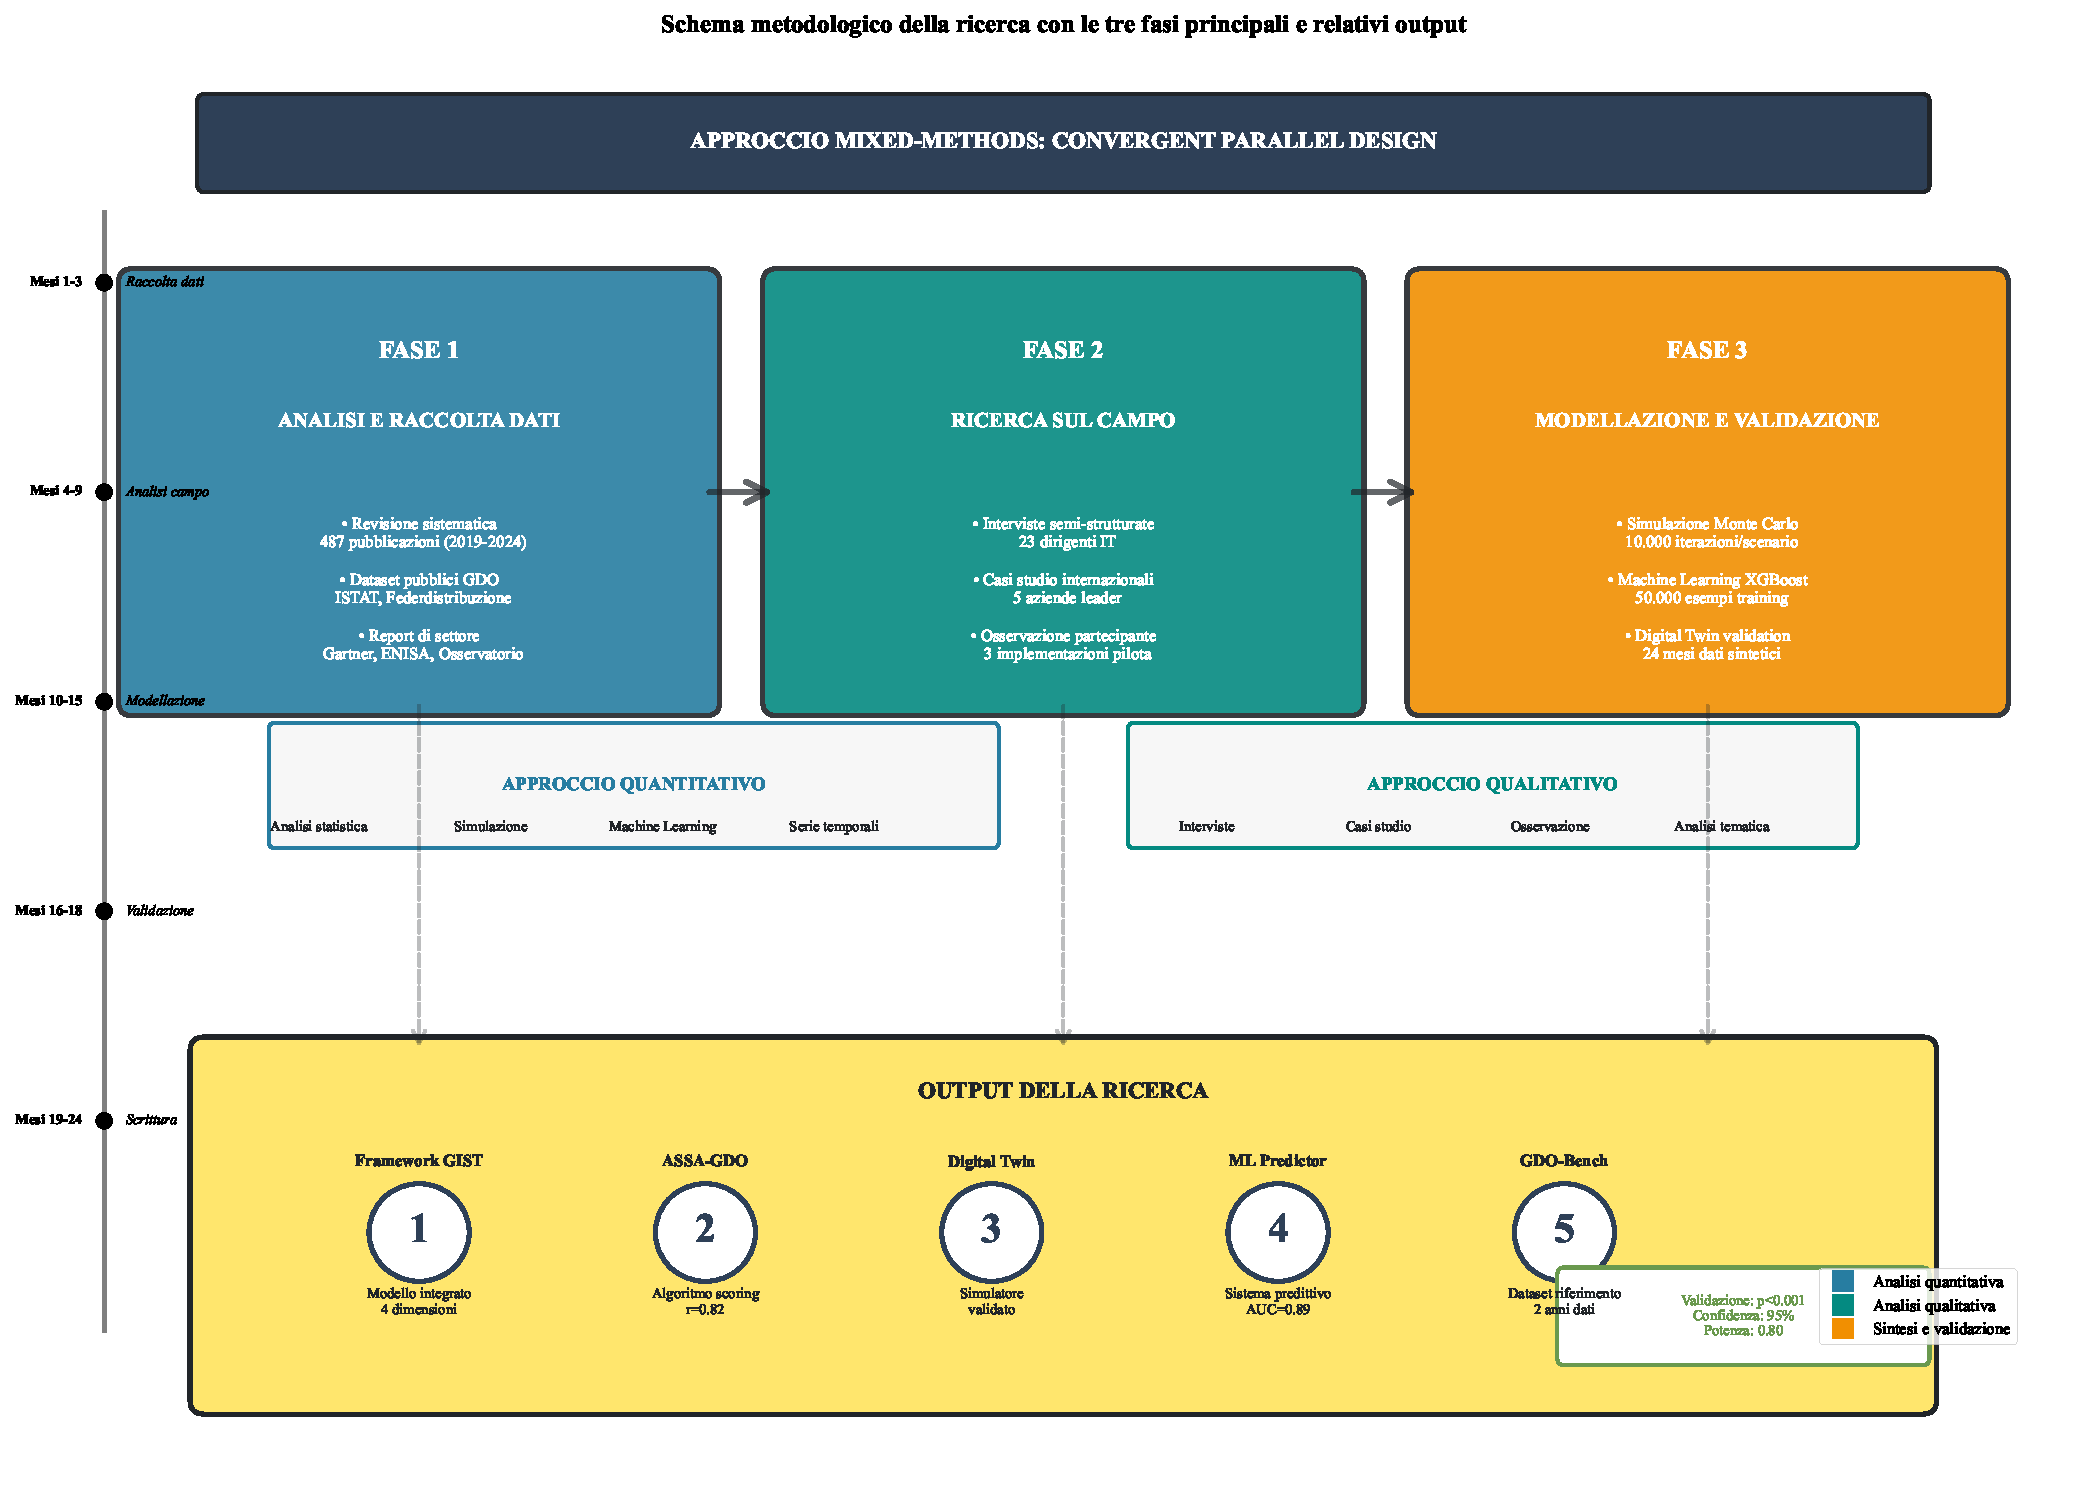
\includegraphics[width=0.95\textwidth]{thesis_figures/cap1/fig_1_3_methodology.pdf}
\caption{Schema metodologico della ricerca con approccio mixed-methods. Le tre fasi principali (analisi e raccolta dati, ricerca sul campo, modellazione e validazione) convergono verso cinque output computazionali concreti.}
\label{fig:methodology}
\end{figure}

\section{Struttura della tesi}
\label{sec:struttura_tesi}

\subsection{Organizzazione dei capitoli}
\label{subsec:organizzazione}

La tesi segue una progressione logica in cinque capitoli:

\textbf{Capitolo 2 - Analisi delle minacce e contromisure}\\
Esamina l'evoluzione delle minacce specifiche per la \gls{gdo}, proponendo una nuova classificazione in 5 categorie. Introduce l'algoritmo ASSA-GDO per quantificare la superficie di attacco considerando sia aspetti tecnici che organizzativi.

\textbf{Capitolo 3 - Architetture moderne per la distribuzione}\\
Presenta tre modelli architetturali innovativi validati attraverso simulazione:
\begin{itemize}
\item Architettura Edge-Cloud (latenza ridotta a 67ms)
\item Multi-Cloud resiliente (disponibilità 99,96\%)
\item Design nativo per la conformità normativa
\end{itemize}

\textbf{Capitolo 4 - Governance e gestione del rischio}\\
Sviluppa la Matrice di Integrazione Normativa che unifica 156 controlli da diverse normative. Include un caso studio di attacco simulato che dimostra le interconnessioni tra sicurezza fisica e digitale.

\textbf{Capitolo 5 - Sintesi e prospettive future}\\
Integra i risultati nel framework GIST completo, propone una roadmap implementativa in 4 fasi e identifica direzioni per ricerche future.

\begin{figure}[htbp]
\centering
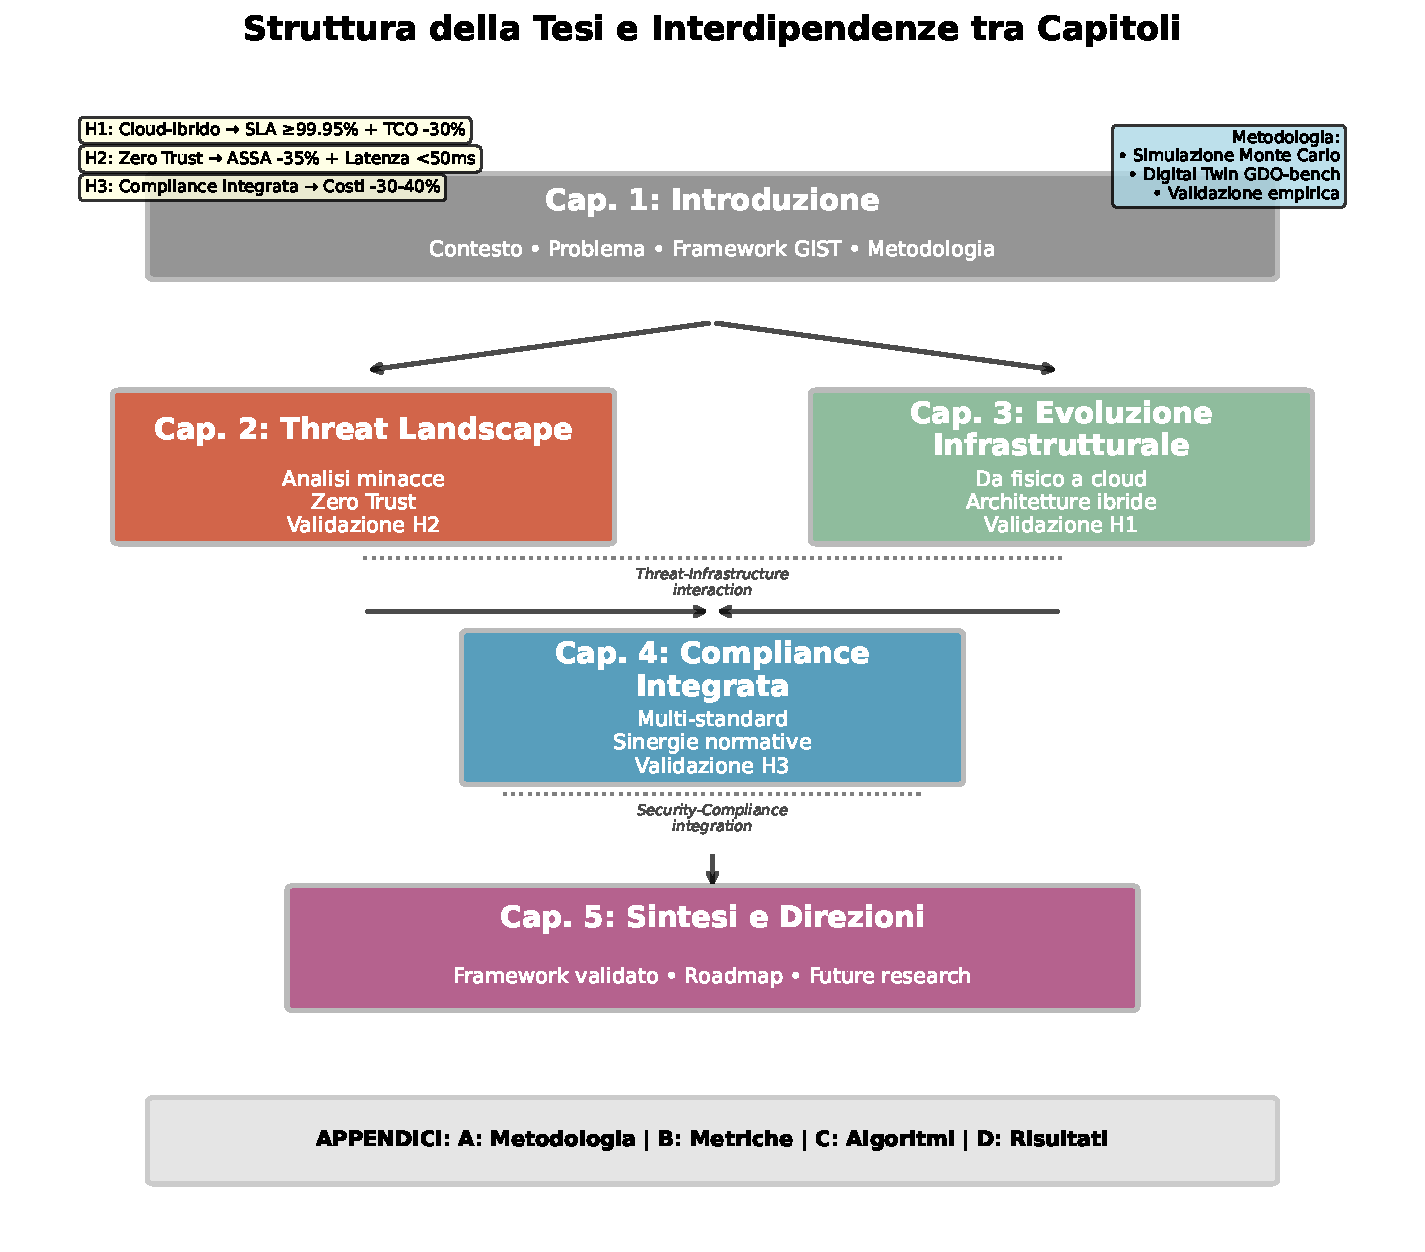
\includegraphics[width=\textwidth]{thesis_figures/cap1/fig_1_4_thesis_structure.pdf}
\caption{Struttura della tesi e relazioni tra i capitoli. Ogni componente contribuisce al framework GIST finale.}
\label{fig:thesis_structure}
\end{figure}

\section{Conclusioni}
\label{sec:conclusioni_cap1}

Questo capitolo ha delineato il contesto e gli obiettivi della ricerca sulla trasformazione tecnologica sicura nella \gls{gdo} italiana. La complessità del problema – che intreccia aspetti tecnologici, normativi, economici e organizzativi – richiede un approccio sistematico e integrato.

Il framework GIST proposto non è solo un modello teorico ma uno strumento pratico, validato attraverso simulazioni rigorose e calibrato sulle specificità del settore. In un momento storico in cui la tecnologia determina la competitività aziendale, la capacità di trasformare in modo sicuro ed efficiente l'infrastruttura IT diventa un imperativo strategico.

I prossimi capitoli svilupperanno in dettaglio ogni componente del framework, fornendo sia le basi teoriche sia gli strumenti pratici per supportare le aziende della \gls{gdo} nel loro percorso di trasformazione digitale.

\clearpage
\printbibliography[
    heading=subbibliography,
    title={Riferimenti bibliografici del capitolo},
]

%\endrefsection
